\section{Description of the prototype and the experimental setup} \label{sec:description_experiment}
The FOWTC hull concept is the result of the parametrical optimization procedure reported by \citet{mas2022parametric}. Following the two objectives given in Section~\ref{sec:introduction}, the experiments were conducted in such a way that they were as close as possible to the design conditions in order to allow for the verification of the numerical methods. Two main differences are, however, present: the water depth, which had to be reduced from $600\,\text{m}$ to $233\,\text{m}$, and the limitations of the software-in-the-loop approach, outlined in Section~\ref{sec:introduction} and discussed in details in Section~\ref{sec:impact_simplifications}.

The experimental campaign was conducted at the wave basin of the Numerical Offshore Tank of the University of São Paulo (TPN-USP), a squared $14\,\text{m}\times 14\,\text{m} \times 4\,\text{m}$ (length, width, depth) tank equipped with 152 active-absorption flap-type wave generators that is shown in Figure~\ref{fig:description_experiment:tanque}.
\begin{figure}[!hbtp]
	\centering
	\includegraphics[width=0.5\columnwidth]{./figures/CH-tpn.jpg}%
	\caption{Wave basin of the Numerical Offshore Tank of the University of São Paulo.} \label{fig:description_experiment:tanque}%
\end{figure}%


\subsection{Main properties of the FOWTC}
%- Caracteristicas da FOWT, RNA, ancoragem
The FOWTC concept consists of a semi-submersible hull with a $14.1\,\text{m}$ diameter central column attached to three $17.0\,\text{m}$ diameter columns arranged as an equilateral triangle, connected by rectangular pontoons $17.0\,\text{m}$ high and $6.0\,\text{m}$ wide, which was built in a 1:60 scale for the experiments. 

During design, the RNA of the IEA 15MW turbine \citep{gaertner2020definition} and the tower of the UMaine VolturnUS-S floater~\citep{allen2020definition} were considered to be mounted on top of the central column. However, their inertial and structural characteristics were not preserved during the tests, specially because the inertia of the rotor, which is mainly due to the blades, was replaced by a set of fans that is way lighter than it should. Instead, the global inertial properties of the whole FOWT were matched by using a ballast system that included a moving set of weights that could be adjusted along a fuse located on top of the tower, as shown in the picture of the model given in Figure~\ref{fig:description_experiment:modelo}. The main properties of the model are listed in Table~\ref{tab:description_experiment:FOWTC_properties}, with the values corresponding to the ones that were measured from the model. Note that since rotor inertia is not reproduced, gyroscopic loads induced by motions of the spinning rotor are not included in the tests, and this is one of the reasons why some researchers have been working on SIL approaches that are able to reproduce loads besides the aerodynamic thrust.
\begin{figure}[!hbtp]
	\centering
	\includegraphics[height=8cm]{./figures/foto_modelo.png}%
\hspace{12pt}    
    \includegraphics[height=8cm]{./figures/foto_mooring.png}%
	\caption{Pictures of the FOWTC model, including an underwater view showing the moorings.} \label{fig:description_experiment:modelo}%
\end{figure}%
%\begin{figure}[!hbtp]
%	\centering
%	\fbox{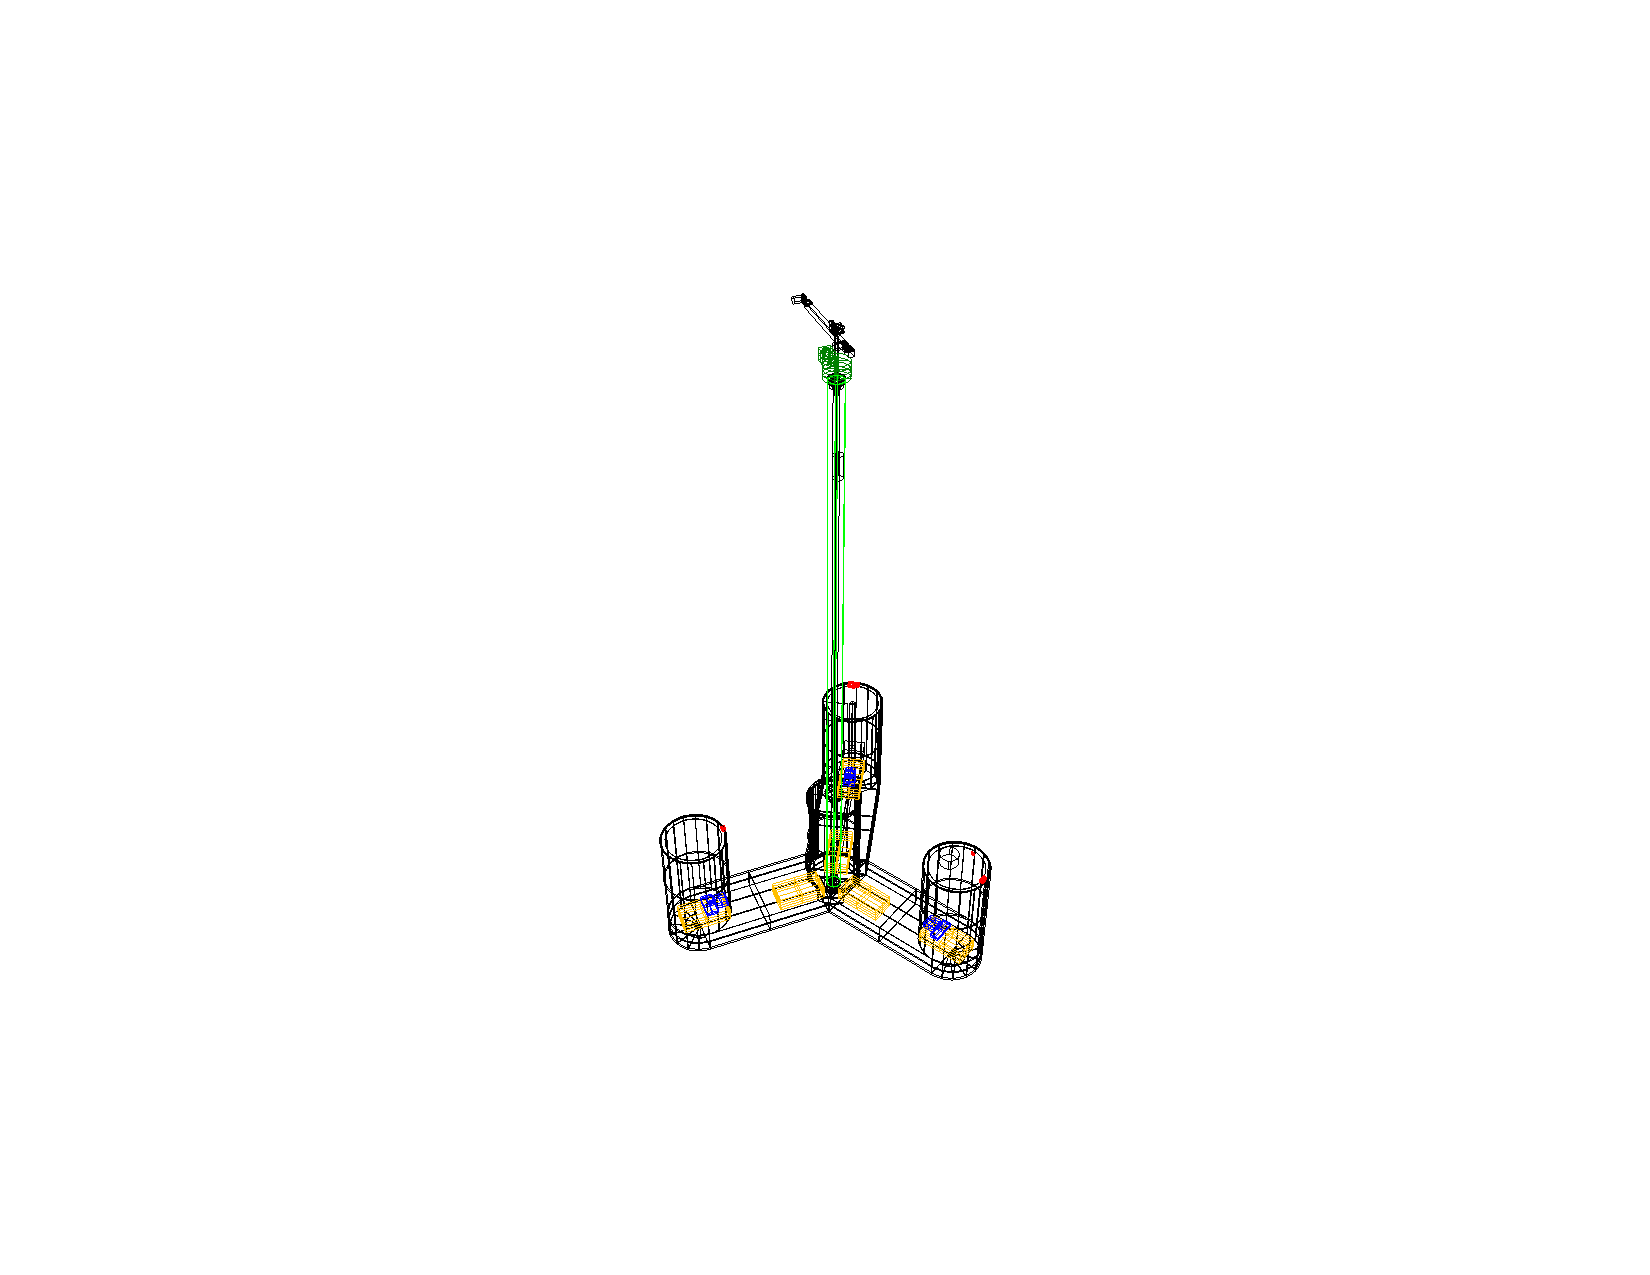
\includegraphics[trim={11cm 5cm 11cm 5cm},clip, height=10cm]{./figures/rhino_lastros.pdf}}%
%	\caption{Picture of the FOWTC model.} \label{fig:description_experiment:rhino_lastros}%
%\end{figure}%

\begin{table}[pos=h]
	\centering
	\caption{Main properties of the FOWTC.}\label{tab:description_experiment:FOWTC_properties}
    %\resizebox{\columnwidth}{!}{%
	\begin{tabular}{lrr}
		\toprule
		& Full scale & Model Scale (1:60) \\
		\midrule
		Mass & $22 \mkern2mu 227 \, \text{t}$ & $102.9 \, \text{kg}$\\
		%
		Displacement & $23 \mkern2mu 120 \, \text{m}^3$ & $107.0 \, \text{L}$\\
		%
		Diam. of central column & $ 14.1 \, \text{m}$ & $233\,\text{mm}$ \\
		%
		Diam. of side columns & $ 17.0 \, \text{m}$ & $283\,\text{mm}$ \\
        %
		Width of pontoons & $ 17.0 \, \text{m}$ & $283\,\text{mm}$ \\
        %
		Height of pontoons & $ 6.0 \, \text{m}$ & $100\,\text{mm}$ \\
		%
		Pitch/roll gyradius$^\dagger{}$ & $44.7 \, \text{m}$ & $745\,\text{mm}$ \\
		%
		Yaw gyradius$^\dagger{}$ & $29.1 \, \text{m}$ & $485\,\text{mm}$\\
		%
		Draft & $18.1 \, \text{m}$ & $301\,\text{mm}$ \\
		%
		KG & $18.4 \, \text{m}$ & $306 \,\text{mm}$ \\		
		%
		GM & $10.72 \, \text{m}$ & $179 \,\text{mm}$  \\
        \bottomrule
        & & \\[-2pt]
		%
        \toprule
        \multicolumn{3}{l}{Natural periods$^\ddagger{}$} \\ 
		\midrule        
		Surge/Sway & $156.9 \,\text{s}$ & $20.3 \,\text{s}$ \\
		Heave & $16.5 \,\text{s}$ & $2.1 \,\text{s}$ \\
		Pitch/Roll & $28.8 \,\text{s}$  & $3.7 \,\text{s}$\\
		Yaw & $79.4 \,\text{s}$ & $10.3 \,\text{s}$\\
		\bottomrule
        \multicolumn{3}{l}{$^\dagger{}$ {\small About global center of mass.}} \\ 
        \multicolumn{3}{l}{$^\ddagger{}$ {\small Obtained from decay tests of the moored model.}}
	\end{tabular}%
    %}
\end{table}%

The model was moored using three catenary mooring lines made of chain (bottom) and polyethylene (upper) segments, with the upper segment being so light that it was not possible to evaluate its weight using the available equipment (this led the need of a workaround in the numerical model, as explained in Section~\ref{sec:numerical_models}). The fairleads were located on the outer side of the side columns, thus $46.7\,\text{m}$ distant from the axis of the central column and with an angular distribution of 120\textdegree{} between them, and fitted with dynamometers to measure line tension. The anchors were attached on top of horizontal plates that were needed due to the presence of a rotating arm located on the bottom of the wave basin, as shown in Figure~\ref{fig:description_experiment:modelo}, thus resulting in a water depth of $233\,\text{m}$. The main characteristics of the mooring system are summarized in Table~\ref{tab:description_experiment:mooring_properties}. 
\begin{table}[!hbtp]
	\centering
	\caption{Main properties of the mooring system.} \label{tab:description_experiment:mooring_properties}
    %\resizebox{\columnwidth}{!}{%
	\begin{tabular}{lrr}
		\toprule
		& Full scale & Model scale (1:60)\\
		\midrule
		Anchors depth & $233.0\,\text{m}$ & $3\mkern2mu883 \, \text{mm}$\\
		Anchors radius from center & $411.0 \, \text{m}$ & $6\mkern2mu850 \, \text{mm}$\\
		\midrule
		Fairleads depth & $18.1 \, \text{m}$ &  $302 \, \text{mm}$\\
		Fairleads radius & $46.7 \, \text{m}$ &  $778 \, \text{mm}$\\
		\midrule
		Bottom segment material & Chain & Chain\\
		Length &  $423.8 \, \text{m}$ & $7\mkern2mu063 \, \text{mm}$\\
		Mass density & $1068 \, \text{kg}/\text{m}$ & $0.297 \, \text{kg}/\text{m}$ \\
		Volume-equivalent diameter & $0.40\,\text{m}$ & $7\,\text{mm}$ \\
		Adopted drag coefficient & $1.6$ & $1.6$	\\
		\midrule
		Upper segment material & Polyethylene & Polyethylene$^\dagger$\\
		Length & $45 \, \text{m}$  & $75 \, \text{mm}$\\
		Mass density & \multicolumn{2}{r}{Too light to measure} \\
		Volume-equivalent diameter & $0.06\,\text{m}$ & $1\,\text{mm}$ \\
		Adopted drag coefficient & $1.6$ & $1.6$ \\
		\bottomrule        
        \multicolumn{3}{l}{\footnotesize $^\dagger $More specifically, a multifilament polyethylene braided fishing line.}
	\end{tabular}%
    %}
\end{table}%


\subsection{Software-in-the-loop approach for aerodynamic loads}
Tem que incluir o controle. Adicionar alguns resultados de teste de bancada?



\subsection{Environmental conditions} \label{sec:description_experiment:envir}
- Condições de onda e vento